\documentclass{beamer}\usepackage[]{graphicx}\usepackage[]{color}
%% maxwidth is the original width if it is less than linewidth
%% otherwise use linewidth (to make sure the graphics do not exceed the margin)
\makeatletter
\def\maxwidth{ %
  \ifdim\Gin@nat@width>\linewidth
    \linewidth
  \else
    \Gin@nat@width
  \fi
}
\makeatother

\definecolor{fgcolor}{rgb}{1, 0.894, 0.769}
\newcommand{\hlnum}[1]{\textcolor[rgb]{0.824,0.412,0.118}{#1}}%
\newcommand{\hlstr}[1]{\textcolor[rgb]{1,0.894,0.71}{#1}}%
\newcommand{\hlcom}[1]{\textcolor[rgb]{0.824,0.706,0.549}{#1}}%
\newcommand{\hlopt}[1]{\textcolor[rgb]{1,0.894,0.769}{#1}}%
\newcommand{\hlstd}[1]{\textcolor[rgb]{1,0.894,0.769}{#1}}%
\newcommand{\hlkwa}[1]{\textcolor[rgb]{0.941,0.902,0.549}{#1}}%
\newcommand{\hlkwb}[1]{\textcolor[rgb]{0.804,0.776,0.451}{#1}}%
\newcommand{\hlkwc}[1]{\textcolor[rgb]{0.78,0.941,0.545}{#1}}%
\newcommand{\hlkwd}[1]{\textcolor[rgb]{1,0.78,0.769}{#1}}%
\let\hlipl\hlkwb

\usepackage{framed}
\makeatletter
\newenvironment{kframe}{%
 \def\at@end@of@kframe{}%
 \ifinner\ifhmode%
  \def\at@end@of@kframe{\end{minipage}}%
  \begin{minipage}{\columnwidth}%
 \fi\fi%
 \def\FrameCommand##1{\hskip\@totalleftmargin \hskip-\fboxsep
 \colorbox{shadecolor}{##1}\hskip-\fboxsep
     % There is no \\@totalrightmargin, so:
     \hskip-\linewidth \hskip-\@totalleftmargin \hskip\columnwidth}%
 \MakeFramed {\advance\hsize-\width
   \@totalleftmargin\z@ \linewidth\hsize
   \@setminipage}}%
 {\par\unskip\endMakeFramed%
 \at@end@of@kframe}
\makeatother

\definecolor{shadecolor}{rgb}{.97, .97, .97}
\definecolor{messagecolor}{rgb}{0, 0, 0}
\definecolor{warningcolor}{rgb}{1, 0, 1}
\definecolor{errorcolor}{rgb}{1, 0, 0}
\newenvironment{knitrout}{}{} % an empty environment to be redefined in TeX

\usepackage{alltt}
\usepackage{../371g-slides}
% Uncomment these lines to print notes pages
% \pgfpagesuselayout{4 on 1}[letterpaper,border shrink=5mm,landscape]
% \setbeameroption{show only notes}
\title{Inference for simple regression 1}
\subtitle{Lecture 3}
\author{STA 371G}
\IfFileExists{upquote.sty}{\usepackage{upquote}}{}
\begin{document}
  
  
  

  \frame{\maketitle}

  % Show outline at beginning of each section
  \AtBeginSection[]{
    \begin{frame}<beamer>
      \tableofcontents[currentsection]
    \end{frame}
  }

  %%%%%%% Slides start here %%%%%%%

  \begin{darkframes}
    \begin{frame}{Announcements and logistics}
      \begin{itemize}[<+->]
        \item Reminder: Pretest due at Thursday 11:59 PM
        \item The course help site (``Lecture slides and R help'' on the left side of Canvas) now has review advice and links to review videos
        \item Course help site also has lecture slides and scripts, and slides, scripts, and videos from Tuesday night R help sessions
        \item The ``Class kickoff survey'' closes tomorrow night; please complete it before then in Learning Catalytics to let me know of your previous experience (and so I can send you a free MyStatLab access code if you previously bought the 3rd edition of the book)
      \end{itemize}
    \end{frame}

    \begin{frame}{Measuring goodness-of-fit}
      \begin{itemize}[<+->]
        \item $R^2$ measures the fraction of the variation in $Y$ explained by $X$;
        in our analysis from last time, $R^2=0.03$.
        \item The \alert{standard error of the regression} $s_e$ can be roughly interpreted as
        the standard deviation of the residuals.
      \end{itemize}
    \end{frame}

    \begin{frame}{Interpreting the standard error of the regression $s_e = 2.96$}
      \begin{itemize}[<+->]
        \item The \alert{residual} for the $i$th case is $Y_i - \hat Y_i$
        \item The residuals are approximately Normally distributed
        \item The mean of the residuals is 0 (why?)
        \item Therefore: 95\% of the residuals are roughly within $\pm 2 s_e$
        \item In other words, 95\% of the time I expect my prediction to be off by at most $5.93$
      \end{itemize}
    \end{frame}

    \begin{frame}
      In our regression, $R^2=0.03$.

      Is this ``significant?''
      \pause
      \begin{itemize}[<+->]
        \item \textbf{Statistical significance:} Can we reject the null hypothesis that the correlation between $X$ and $Y$ in the \emph{population} is zero?
        \item \textbf{Practical significance:} Is the relationship in our sample strong enough to be meaningful?
      \end{itemize}
    \end{frame}

    \begin{frame}{The overall null hypothesis for a regression model}
      The following are equivalent ways to express the overall null hypothesis:
      \begin{itemize}[<+->]
        \item $R^2=0$ (in the population)
        \item $\text{cor}(X,Y)=0$ (in the population)
        \item $\beta_1=0$
        \item The model has no predictive power
        \item Predictions from this model are no better than predicting $\overline Y$ for every case
      \end{itemize}
    \end{frame}

    \begin{frame}{Two ways to test the overall null hypothesis}
      \begin{itemize}
        \item The $F$-test (tests $H_0:R^2=0$ in the population vs $H_A:R^2\neq 0$)
        \item The $t$-test for the \emph{slope} ($\beta_1$) coefficient (tests $H_0:\beta_1=0$ vs $H_A:\beta_1\neq 0$)
        \item Note that both tests are two-tailed, since we would care about the null hypothesis being wrong in either direction (i.e. $\beta_1>0$ and $\beta_1<0$ are both of interest)
      \end{itemize}
      \pause
      Both of these methods are equivalent; the $p$-values will be exactly the same!
    \end{frame}

    \begin{frame}[fragile]
      \note{Point out where these $p$-values are found on the R output.}
      \fontsize{9}{9}\selectfont
\begin{knitrout}
\definecolor{shadecolor}{rgb}{0.137, 0.137, 0.137}\begin{kframe}
\begin{alltt}
\hlstd{> }\hlstd{model} \hlkwb{<-} \hlkwd{lm}\hlstd{(num.drinks} \hlopt{~} \hlstd{age)}
\hlstd{> }\hlkwd{summary}\hlstd{(model)}
\end{alltt}
\begin{verbatim}

Call:
lm(formula = num.drinks ~ age)

Residuals:
   Min     1Q Median     3Q    Max 
-4.204 -1.853 -0.853  0.810 15.160 

Coefficients:
            Estimate Std. Error t value Pr(>|t|)    
(Intercept)   6.5542     0.2653    24.7   <2e-16 ***
age          -0.1688     0.0159   -10.6   <2e-16 ***
---
Signif. codes:  0 '***' 0.001 '**' 0.01 '*' 0.05 '.' 0.1 ' ' 1

Residual standard error: 3 on 3600 degrees of freedom
  (2902 observations deleted due to missingness)
Multiple R-squared:  0.0304,	Adjusted R-squared:  0.0302 
F-statistic:  113 on 1 and 3600 DF,  p-value: <2e-16
\end{verbatim}
\end{kframe}
\end{knitrout}
    \end{frame}

    \begin{frame}{What is our conclusion about $\beta_1$?}
      \begin{itemize}[<+->]
        \item There is a \textbf{statistically significant} relationship between the age someone starts drinking and how much they drink as an adult.
        \item Or: People that start drinking earlier in life consume \textbf{significantly more} alcohol when they drink as adults.
        \item Each additional year you wait to start drinking is associated with consuming 0.17 fewer drinks as an adult.
        \item Is this relationship \textbf{practically significant}?
      \end{itemize}
    \end{frame}

    \begin{frame}{Practical significance}
      \begin{itemize}
        \item To assess \textbf{statistical significance}, we look at the $p$-value
        \item To assess \textbf{practical significance}:
          \begin{itemize}
            \item We only consider it if we already have statistical significance (why?)
            \item Look at $R^2$, the standard error of the regression, and the magnitude of the coefficients
            \item It's ultimately a judgement call!
          \end{itemize}
      \end{itemize}
    \end{frame}

    \begin{frame}{Put a confidence interval on it}
      \begin{itemize}[<+->]
        \item Our best estimate for the \emph{effect} of a year's postponement of drinking is 0.17 fewer drinks as an adult
        \item We can use a confidence interval to give a range of plausible values for what this effect size is in the population
      \end{itemize}
    \end{frame}

    \begin{frame}[fragile]{Put a confidence interval on it}
      A confidence interval is always of the form \[ \text{estimate} \pm (\text{critical value})(\text{standard error}). \]
      \pause
      Recall that the critical value for a 95\% confidence interval is the cutoff value that cuts off 95\% of the area in the middle of the distribution; the sampling distribution of $\hat\beta_1$ is a $t$-distribution.


\begin{knitrout}
\definecolor{shadecolor}{rgb}{0.137, 0.137, 0.137}\begin{kframe}
\begin{alltt}
\hlstd{> }\hlstd{n} \hlkwb{<-} \hlkwd{nobs}\hlstd{(model)}
\hlstd{> }\hlkwd{qt}\hlstd{(}\hlnum{0.975}\hlstd{, n}\hlopt{-}\hlnum{2}\hlstd{)}
\end{alltt}
\begin{verbatim}
[1] 1.960623
\end{verbatim}
\end{kframe}
\end{knitrout}
    \end{frame}

    \begin{frame}[fragile]{Put a confidence interval on it}
      R will also calculate confidence intervals for us:
\begin{knitrout}
\definecolor{shadecolor}{rgb}{0.137, 0.137, 0.137}\begin{kframe}
\begin{alltt}
\hlstd{> }\hlkwd{confint}\hlstd{(model)}
\end{alltt}
\begin{verbatim}
                 2.5 %     97.5 %
(Intercept)  6.0339847  7.0743549
age         -0.1999713 -0.1376959
\end{verbatim}
\end{kframe}
\end{knitrout}

      \pause
      In other words, we are 95\% confident that the effect of each additional year's delay in starting to drink is between 0.14 and 0.2.
    \end{frame}

    \begin{frame}{Put a confidence interval on it, part 2}
      We can also put a confidence interval on a prediction!

      Two kinds of intervals:
      \bigskip

      \begin{tabular}{lp{1in}p{2in}}
        \textbf{Confidence} & Predicting the mean value of $Y$ for a particular $X$. & Among all people that start drinking at age 21, how many drinks do have on average as adults? \\
        \textbf{Prediction} & Predicting $Y$ for a single new case. & If Bob started drinking at age 21, how many drinks do we think will have as an adult? \\
      \end{tabular}
    \end{frame}

    \begin{frame}[fragile]{Put a confidence interval on it, part 2}

\begin{knitrout}
\definecolor{shadecolor}{rgb}{0.137, 0.137, 0.137}\begin{kframe}
\begin{alltt}
\hlstd{> }\hlkwd{predict}\hlstd{(model,} \hlkwd{list}\hlstd{(}\hlkwc{age}\hlstd{=}\hlnum{21}\hlstd{),}
\hlstd{+ }  \hlkwc{interval}\hlstd{=}\hlstr{'confidence'}\hlstd{)}
\end{alltt}
\begin{verbatim}
       fit     lwr      upr
1 3.008664 2.83616 3.181167
\end{verbatim}
\begin{alltt}
\hlstd{> }\hlkwd{predict}\hlstd{(model,} \hlkwd{list}\hlstd{(}\hlkwc{age}\hlstd{=}\hlnum{21}\hlstd{),}
\hlstd{+ }  \hlkwc{interval}\hlstd{=}\hlstr{'prediction'}\hlstd{)}
\end{alltt}
\begin{verbatim}
       fit       lwr      upr
1 3.008664 -2.802894 8.820221
\end{verbatim}
\end{kframe}
\end{knitrout}

      \pause
      Why is the prediction interval wider?
      \lc
    \end{frame}

    \begin{frame}
      \fullpagepicture{xkcd}
    \end{frame}

    \begin{frame}{Correlation $\neq$ Causation}
      Because the $p$-value is small, we can be highly confident that there is a relationship in
      the population between age of first drink and number of drinks consumed as an adult.

      \bigskip
      This could be because:

      \pause

      \begin{itemize}[<+->]
        \item Starting to drink earlier causes you to drink more as an adult.
        \item Being predisposed to drink more will cause you to start drinking sooner.
        \item There is a third (``lurking'') variable that causes both early drinking and drinking more as an adult.
      \end{itemize}

      \pause
      We can't tell just by looking at this data set!
    \end{frame}

    \begin{frame}
      \begin{center}
        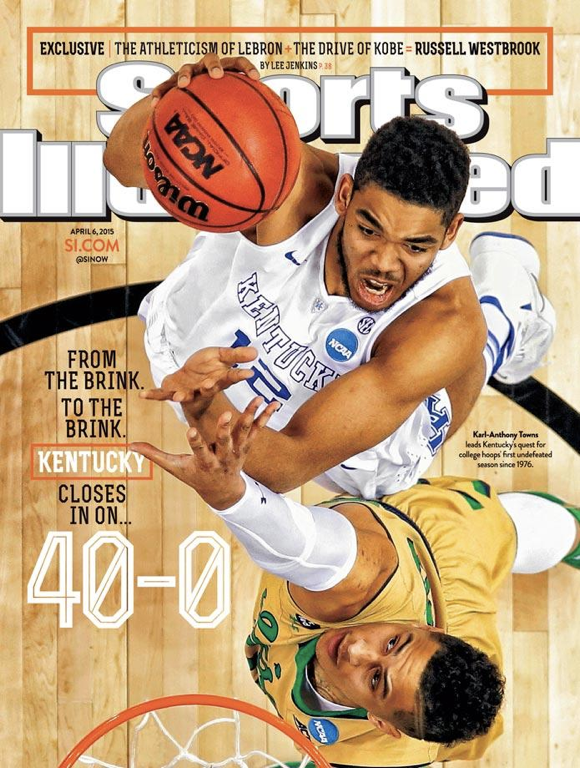
\includegraphics[width=2.5in]{si}
      \end{center}
    \end{frame}

    \begin{frame}{Regression to the mean}
      The value of $Y$ will tend to be closer to the mean than $X$, on average (even if you switch $X$ and $Y$!).
      \begin{itemize}
        \item Students who take the SAT again after getting a very low score tend to improve even if they don't receive any coaching
        \item Children of tall parents tend to be tall, but not as tall as their parents
        \item Olympic champions tend to have poorer performances following their Olympic victories
        \item The ``\emph{Sports Illustrated} curse'' of athletes that appear on the cover
      \end{itemize}
    \end{frame}

    \begin{frame}{Regression to the mean}
      \begin{columns}[onlytextwidth]
        \column{.45\textwidth}
          \begin{itemize}
            \item In this graph, variables have been standardized, $r=0.8$, and $\hat Y = 0.8X$
            \item Parent at mean $\to$ predict child height is also at the mean
            \item Parent 1 SD above mean $\to$ predict child height 0.8 SD above the mean
            \item Parent 2 SD above mean $\to$ predict child height 1.6 SD above the mean
          \end{itemize}
        \column{.5\textwidth}
\begin{knitrout}
\definecolor{shadecolor}{rgb}{0.137, 0.137, 0.137}
\input{/tmp/figures/unnamed-chunk-10-1.tex}

\end{knitrout}
      \end{columns}

    \end{frame}

  \end{darkframes}

\end{document}
